\chapter{Laplace transforms}

\section{Heaviside function}
So far, we have dealt with so-called \textit{nice functions}. Consider the step function:
\[
u(t) =
\begin{cases}
0, \quad t < 0 \\
1, \quad t > 0
\end{cases}
\]

where $u(0)$ is undefined. This function is called the \textbf{Heaviside function}.

\begin{figure}[H]
    \centering
    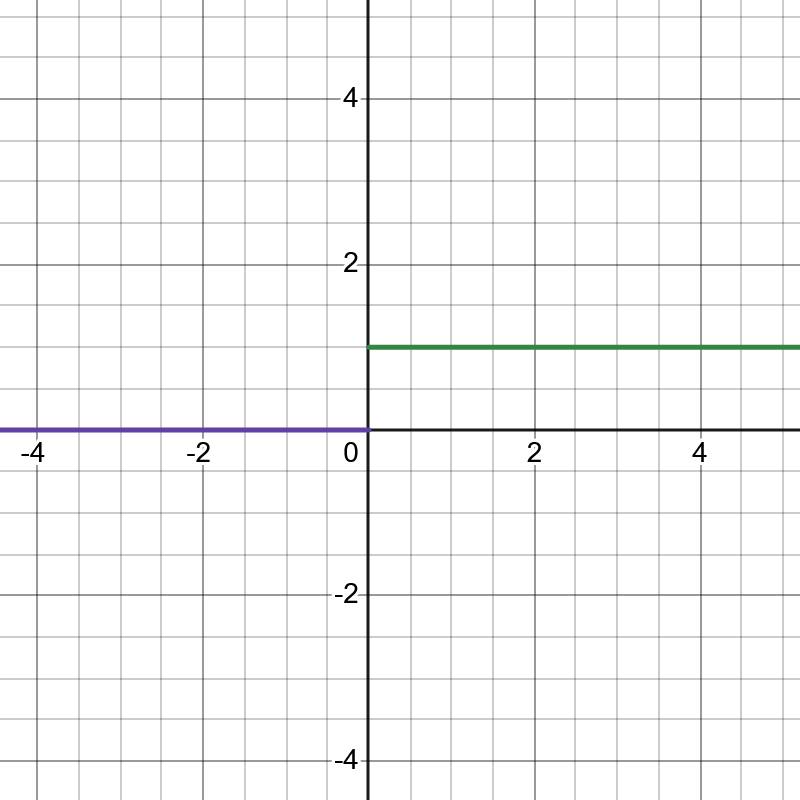
\includegraphics[width=0.5\textwidth]{images/laplace_transforms/heaviside_function.png}
    \caption{Graph of the Heaviside function}
    \label{fig:heaviside}
\end{figure}

We can apply a shift to the Heaviside function such that it "turns on" at $t = a$:
\begin{figure}[H]
    \centering
    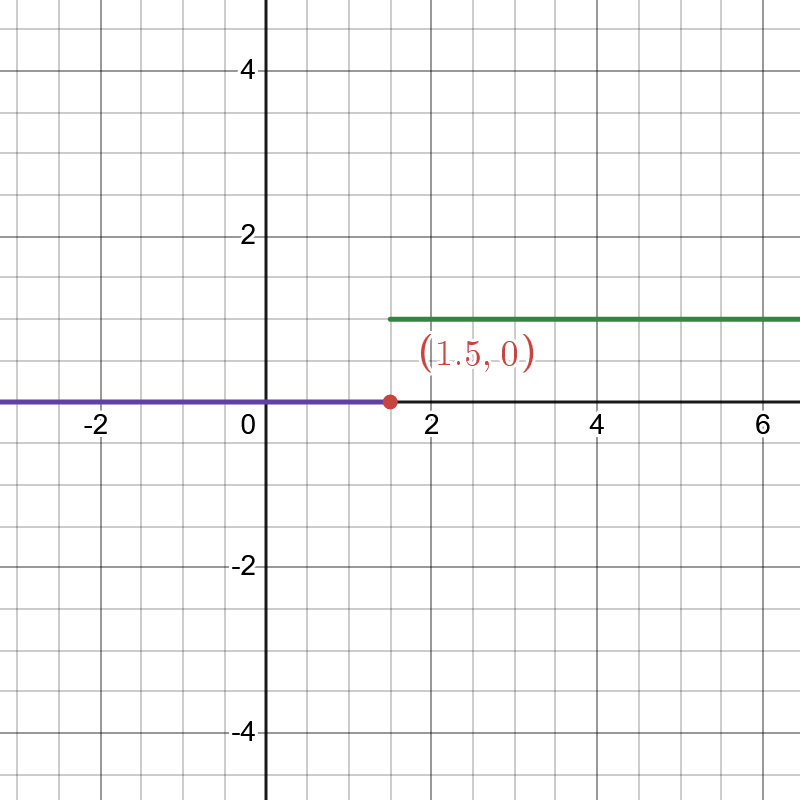
\includegraphics[width=0.5\textwidth]{images/laplace_transforms/heaviside_function_shift.png}
    \caption{Graph of the shifted Heaviside function}
    \label{fig:heaviside_shift}
\end{figure}

Finally, if we take two shifted Heaviside functions such that $a < b$, we get a function that resembles the following:
\begin{figure}[H]
    \centering
    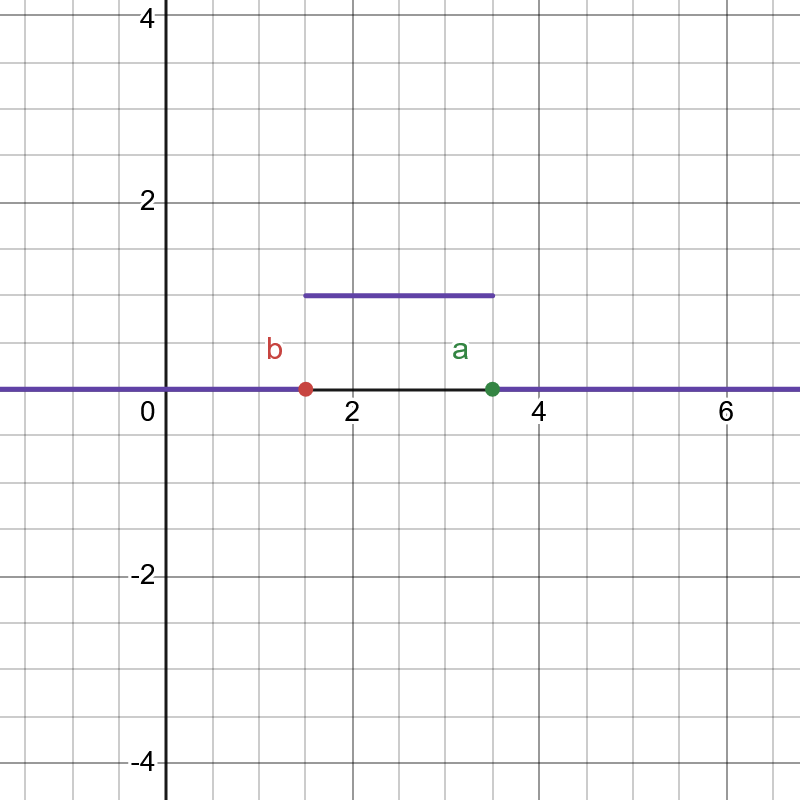
\includegraphics[width=0.5\textwidth]{images/laplace_transforms/heaviside_function_subtract.png}
    \caption{Graph of the shifted Heaviside function}
    \label{fig:heaviside_shift_2}
\end{figure}

We can see that this becomes useful to restrict the range of a function $f(t)$ to a certain interval. If the function is only "on" with $t \in (a, b)$, then we can write $f(t) = f(t)(u(t - a) - u(t - b))$.

\subsection{Bank account example}
Let's assume we have a bank account for which the change in our balance is modeled by the following:
\[
x(t + \Delta t) = x(t) + Ix(t) \Delta t
\]

where $x(t)$ is the amount current in the account, $\Delta t$ is some time over which interest is accumulated, and $I$ is the interest rate.

\textbf{Remark:} This discrete model is extremely similar to Euler's forward method where $f(x + h) = x + h \cdot f(x)$.

At $t = 0$, we have that $\dot{x} = Ix$. That is, the change in our balance is proportional to the amount currently in the account.
Let us define some rate $q(t)$ at which money is deposited into the account. Note that this is distinct from the interest rate $I$ which is constant. Then, we have that $\dot{x} - Ix = q(t)$.  We must now attempt to determine the cumulative total amount of money $Q(t)$ that has been deposite. It is clear that:
\[
\dot{Q} = q(t) \Longrightarrow Q(t) = \int_{0}^{t} q(\overline{t}) d\overline{t}
\]

Now consider the case where a single \$2000 occurs at $t = 1$, while we are also depositing money at a rate of \$1000 per year. 

Intuitively, we would write $Q(t)$ as:
\[
Q(t) = 1000t + 2000u(t - 1)
\]

We note that the Heaviside function is perfect to represent this situation: we "switch on" the deposit at $t = 1$ and the money remains in the account.

However, we are presented with the challenge of differentiating this function to derive $q(t)$. No such function exists for $u(t)$, but there is a "function" (which is actually a distribution) that satisifes the following properties that we'd expect for such a derivative:
\begin{itemize}
\item We know that the integral of this derivative must be equal to 1 to be equivalent to $u(t)$.
\item The derivative must be zero for $t < 0$ since $u(t)$ is constant for $t < 0$, and the derivative must also be zero for $t > 0$ since $u(t)$ is constant for $t > 0$ - the only point at which $u(t)$ is not constant is at $t = 0$.
\end{itemize}

This "function" is called the \textbf{Dirac delta function} $\delta(t)$, and it is defined as follows:
\[
\delta(t) =
\begin{cases}
\infty, \quad t = 0 \\
0, \quad t \neq 0
\end{cases}
\]

In the example above, we have that $q(t) = 1000 + 2000\delta(t - 1)$.

We could even consider a case where at $t = 1$, we deposit \$1000, and at $t = 2$, we withdraw \$500. In this case, we have that $q(t) = 1000\delta(t - 1) - 500\delta(t - 2)$.

In particular, we visualize the Dirac delta function like this:

\begin{figure}[H]
    \centering
    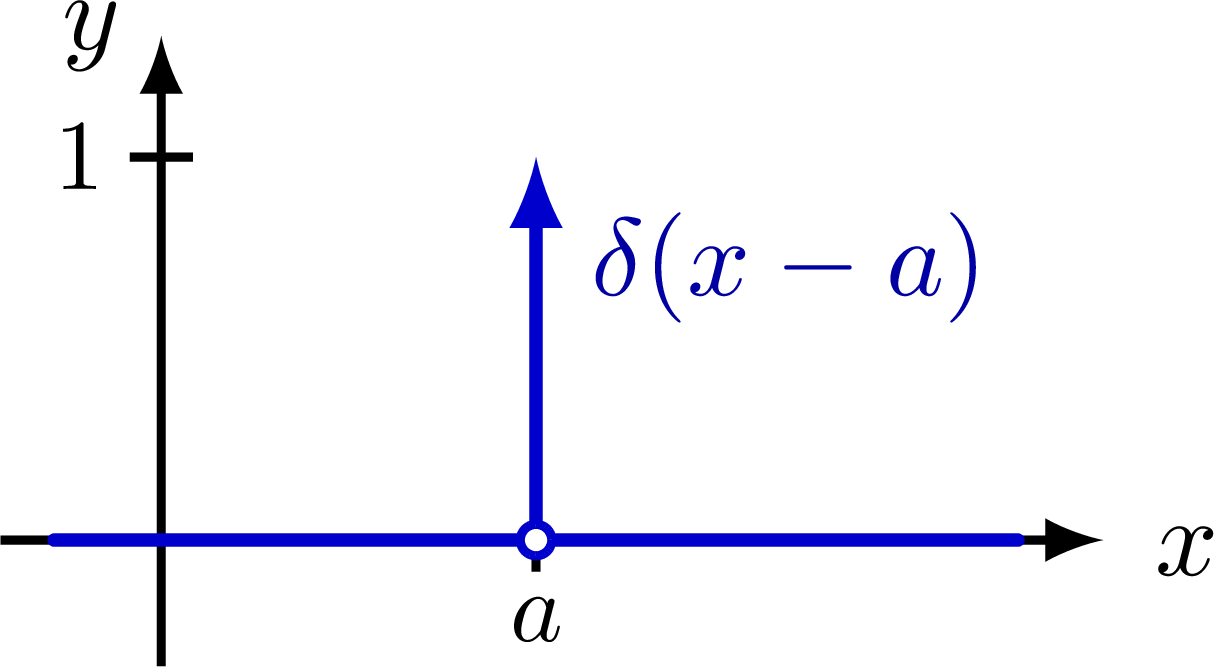
\includegraphics[width=0.5\textwidth]{images/laplace_transforms/dirac_delta_function.png}
    \caption{Graph of the Dirac delta function}
    \label{fig:dirac_delta}
\end{figure}

As convention, we write the $a$ beside the delta function to indicate the integral of the delta function:
\[
\int_{-\infty}^{\infty} a \delta(t) dt = a
\]

Now recall piecewise smooth functions. These functions are broken up into smooth pieces that have limitson the right and on th eleft that exist at each break. These are therefore "nice" functions that switch on or off with different applications of $u(t)$.

For example, consider the function:
\[
f(t) =
\begin{cases}
t, \quad t < 1 \\
1-\sqrt{t}, \quad 1 < t < 2 \\
t-2, \quad t > 2
\end{cases}
\]

This function appears like this:

\begin{figure}[H]
    \centering
    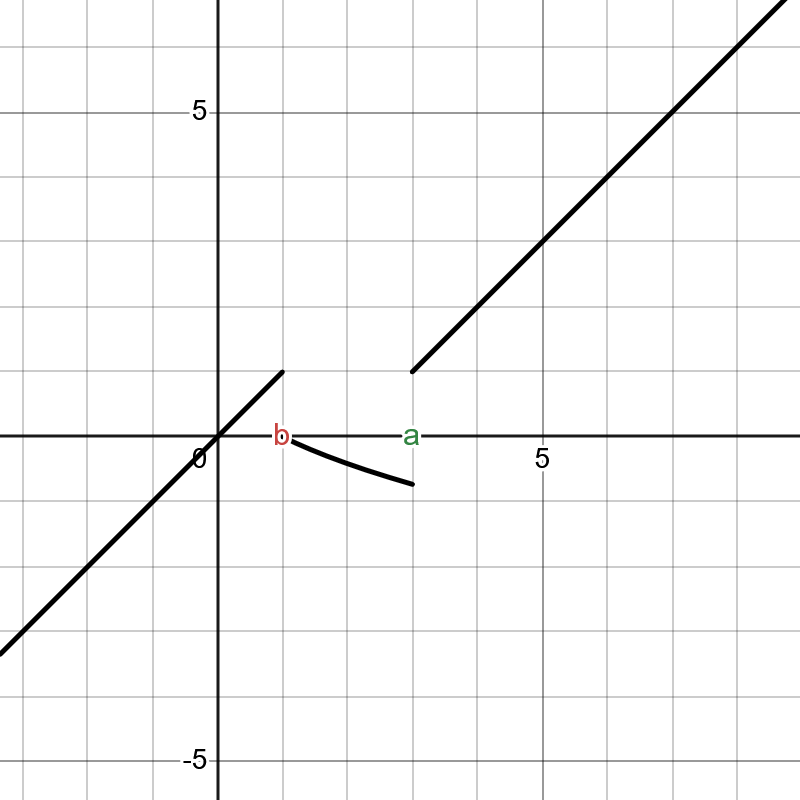
\includegraphics[width=0.5\textwidth]{images/laplace_transforms/piecewise_smooth_function.png}
    \caption{Graph of a piecewise smooth function}
    \label{fig:piecewise_smooth}
\end{figure}

We can write this function in terms of the Heaviside function as follows:
\[
f(t) = t + (1 - \sqrt{t} - t)u(t - 1) + (t - 2 - (1 - \sqrt{t}))u(t - 2)
\]

In general, we can "turn on" a function $f(t)$ at $t = a$ and "turn off" the function at $t = b$ by writing $f(t)(u(t - a) - u(t - b))$. We can also "turn on" a function at $t = a$ and leave it on for all $t > a$ by writing $f(t)u(t - a)$. Then for a piecewise smooth function, we can write it as a sum of functions that are "turned on" at different points. For example, if we have a piecewise smooth function with break points at $t = a_1, a_2, \ldots, a_n$, then we can write the function as:
\[
f(t) = f_1(t) + (f_2(t) - f_1(t))u(t - a_1) + (f_3(t) - f_2(t))u(t - a_2) + \ldots + (f_n(t) - f_{n-1}(t))u(t - a_{n-1})
\]

Basically, at $a_1$, we "turn on" the function $f_2(t)$ with multiplication by $u(t - a_1)$ while the subtraction of $f_1(t) u(t - a_1)$ at the same time "turns off" the function $f_1(t)$, and this process continues for each break point.

\dfn{Generalized derivative}
{
The \textbf{generalized derivative} of a function $f(t)$ is defined as the limit of the difference quotient as $h$ approaches zero, where the difference quotient is given by:
\[
\frac{f(t + h) - f(t)}{h}
\]
This definition allows us to extend the concept of differentiation to functions that may not be differentiable in the traditional sense, such as piecewise smooth functions or functions with discontinuities. The generalized derivative can be used to analyze the behavior of such functions and to solve differential equations that involve them.
}

In particular, given a piecewise smooth function $Q(t)$, we can now find a derivative at point $a$ by:
\[
\dot{Q}(t) = (Q(a^+) - Q(a^-))\delta(t - a)
\]
where $Q(a^+)$ and $Q(a^-)$ are the right and left limits of $Q(t)$ at $t = a$, respectively.

We denote this as:
\[
\boxed{[Q]_a \delta (t - a)}
\]

\ex{Example}{
Consider the function:
\[
Q(t) =
\begin{cases}
0, \quad t < 1 \\
1000t, \quad 1 < t < 2 \\
2000, \quad t > 2
\end{cases}
\]

Find $\dot{Q}(t)$.
}
\sol{
We can write $Q(t)$ in terms of the Heaviside function as follows:
\begin{align*}
Q(t) = 1000t u(t - 1) + (2000 - 1000t)u(t - 2)
= 1000t u(t - 1) + 2000u(t - 2) - 1000t u(t - 2)
\end{align*}

We have three terms to differentiate. 

\begin{align*}
\frac{d}{dt} 1000t u(t - 1) &= 1000u(t - 1) + 1000t \delta(t - 1) \\
\frac{d}{dt} 2000u(t - 2) &= 2000 \delta(t - 2) \\
\frac{d}{dt} 1000t u(t - 2) &= 1000u(t - 2) + 1000t \delta(t - 2)
\end{align*}

Now we can combine these three terms to get:
\begin{align*}
\dot{Q}(t) &= 1000u(t - 1) + 1000t \delta(t - 1) + 2000 \delta(t - 2) - 1000u(t - 2) - 1000t \delta(t - 2) \\
&= 1000u(t - 1) - 1000u(t - 2) + 1000t \delta(t - 1) + (2000 - 1000t) \delta(t - 2)
\end{align*}

Now we use the property that $f(t) = f(a) \delta(t - a)$ to simplify the delta function terms:
\begin{align*}
\dot{Q}(t) &= 1000u(t - 1) - 1000u(t - 2) + 1000t \delta(t - 1) + (2000 - 1000t) \delta(t - 2) \\
&= 1000u(t - 1) - 1000u(t - 2) + 1000 \cdot 1 \cdot \delta(t - 1) + (2000 - 1000 \cdot 2) \delta(t - 2) \\
&= 1000u(t - 1) - 1000u(t - 2) + 1000 \delta(t - 1) + 0 \cdot \delta(t - 2) \\
&= 1000u(t - 1) - 1000u(t - 2) + 1000 \delta(t - 1)
\end{align*}

This can be interpeted as follows: at $t = 1$, we have a deposit of \$1000, which is represented by the delta function term. For $t > 1$, we have a continuous deposit of \$1000 per year, which is represented by the first Heaviside function term. Finally, at $t = 2$, we stop depositing money, which is represented by the second Heaviside function term.
}

Finally, we note that we can shift the delta function as follows:
\begin{equation*}
\delta(t - a) = \frac{d}{dt} u(t - a) 
\end{equation*}

And recalling that:
\begin{equation*}
\int_{-\infty}^{\infty} \delta(t - 1) dt = \int_{-\infty}^{\infty} \delta(t') dt' = 1
\end{equation*}

Applying this to the integral of the delta function multiplied by some function $f(t)$, we have:
\begin{align*}
\int_{-\infty}^{\infty} f(t') \delta (t' - t) dt' &= f(t) \int_{-\infty}^{\infty} \delta(t' - t) dt' \\ 
\end{align*}

We can do this because the delta function is zero everywhere except at $t' = t$, so we can factor out $f(t)$ from the integral. It effectively has a single value, and hence can be treated as a constant. Now, since the integral of the delta function is 1, we have:
\begin{align*}
\int_{-\infty}^{\infty} f(t') \delta (t' - t) dt' &= f(t) \cdot 1 \\
&= f(t)
\end{align*}

